\subsection{Première version 3D}
La première version de l'affichage était simple. Si le vecteur de l'écran rencontrait un obstacle, alors il retournait la couleur RVB avec les composantes égales aux composantes XYZ du vecteur de la normale de l'objet. Sinon, cela signifie que l'on regarde le ciel, auquel cas on retourne un couleur bleue cyan.
\begin{figure}[h]
    \centering
    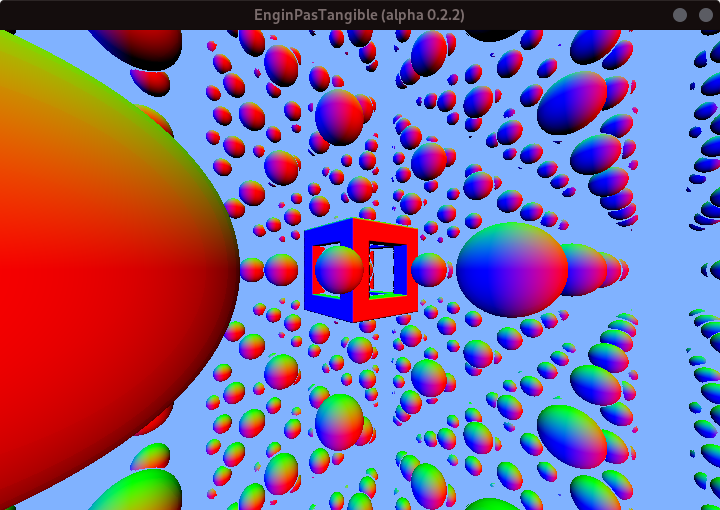
\includegraphics[width=5cm]{images/screens/couleurnormale.png}
    \caption{La couleur des objets est calculée grâce à la direction de la normale}
    \label{fig:firstpreview}
\end{figure}